% Chapter 2

\chapter{Sequential Decision Making under Uncertainty}

\label{chapter2}

%------------------------------------------------------------------------------

% Command definition

%------------------------------------------------------------------------------

\section{Markov Chains \& Concentration Inequalities}

Statistical analysis in real-world processes is often applied to a sequence of random variables, for instance to queues of customers in an airport: given an arrival and a service rates, how many customers do I have in queue at any time? The field of concentration inequalities in particular provides probability tail bounds on the distance from a function of such sequence to its expectation; the most studied case is when the random variables are independent, for which the literature offers many sharp bounds. However, independency is a strong assumption, that isn't always relevant; hence the need to consider other settings. Such are Markov Chains, which model the generation of a sequence of states under what is called the Markov property. It also is a stepping stone towards Markov Decision Processes.

\subsection{Markov Chains}
\label{subsec:MC}

A \emph{Markov Chain} on a countable state space $\mathcal{S}$ is a discrete time stochastic process $X_0, X_1, X_2, \dots \in \mathcal{S}$ satisfying the Markov property. In other words, a Markov Chain moves from one state to another following a transition kernel that is without memory, i.e. only depends on the current state and not on the history before.

\begin{defi}[Markov Property]
  $$\forall (n, s) \in \mathbb{N} \times \mathcal{S},\quad \mathbb{P}(X_{n+1} = s | X_0, \dots, X_n) = \mathbb{P}(X_{n+1} = s | X_n)$$
\end{defi}

A Markov Chain is \textbf{time homogeneous} if the transition probability between two states does not depend on the time $n$. In which case, we have:

\begin{defi}[Transition matrix/kernel] $P: \mathcal{S}^2 \to [0, 1]$ is the transition kernel of $(X_n)_n$ if:
  $$\forall (i, j) \in \mathcal{S}^2,\, \forall n \in \mathbb{N},\quad \mathbb{P}(X_{n+1} = j | X_n = j) = P(i, j)$$
  And if $\mathcal{S}$ is finite, $P = (p_{i, j})_{i, j}$ is the $S \times S$ transition matrix of the Markov Chain.
\end{defi}

Then, one can see that $p_{i, j}^m = \mathbb{P}(X_m = j \,|\, X_0 = i)$, the \emph{$m$-step transition probability}, is the element of the matrix $P^m$ at index $(i, j)$, for all $(i, j, m) \in \mathcal{S}\times \mathcal{S} \times \mathcal{N}$.

Now that the basic concepts have been introduced, let's define some properties of states and Markov Chain, in order to better describe the dynamics behind.

Two states $s, s'$ are said to \emph{communicate} if there exists $m, n \in \mathcal{N}^2$ such that $p_{s, s'}^m > 0$ and $p_{s', s}^n > 0$, i.e. there's a path of non-null probability from $s$ to $s'$ and from $s'$ to $s$. Hence, since the ``communicate'' relation is an equivalence relation, $\mathcal{S}$ can be divided into communication classes. In particular, a Markov Chain is said to be \emph{irreducible} if there is only one communication class, in other words: there exists a path of non-null probability between every pair of states.

To describe how close two states are in the Markov Chain, we define the \emph{hitting time}:
\begin{defi}[Hitting time]
  $$\forall \, s \in \mathcal{S},\quad T^s = \inf \{n \in \mathcal{N}^* \,|\, X_n = i\}$$
  the time of first visit to a state by the Markov Chain.
\end{defi}

Then, depending on the behaviour of the hitting time, a state is said to be \emph{transient} or \emph{recurrent}:
\begin{defi}[Recurrence]
  A state $s \in \mathcal{S}$ is \textbf{recurrent} if and only if
  $$\mathbb{P}(T^s < +\infty \,|\, X_0 = s) = 1$$ otherwise it is \textbf{transient}.\\
  Moreover, if $s$ is recurrent and
  $$\mathbb{E}[T^s \,|\, X_0 = s] < +\infty$$
  then $s$ is said to be \textbf{positive recurrent}, otherwise it is \textbf{null recurrent}.
\end{defi}

In the finite state space case, any recurrent state is positive recurrent. Also, it is interesting to observe that all states in a communication class are either recurrent or transient.

%Furthermore, a state $s$ is said to be \emph{periodic} with period $k \in \mathcal{N}$ if all $m \in \mathcal{N}^*$ such that $p_{s, s}^m > 0$ are divisible by $k$ and $k > 1$. If $k = 1$, then $s$ is \emph{aperiodic}. Again, it is a property shared among a same class.

Finally, we can define \emph{ergodicity}:
\begin{defi}[Ergodicity]\label{ergodicity}
  %A state is ergodic if it is positive recurrent and aperiodic.\\
  %A Markov Chain is ergodic if all states are.\\
  A Markov Chain is ergodic if it is irreducible and positive recurrent.
\end{defi}

Intuitively, in an ergodic Markov Chain all states will be visited regularly and without a periodic pattern. This behaviour is described by the following theorem:
\begin{thm}[Ergodic Theorem]
  Let $P$ be the transition matrix of an ergodic Markov Chain. Then there exists a unique probability distribution $\pi$ over the state space that solves the system of equations $\pi^T = \pi^T P$. $\pi$ is called the \textbf{stationary distribution} of $P$.
\end{thm}

The theorem above motivates the definition of ergodicity: it says that, as time tends towards infinity, the Markov Chain is doomed to fall into steady dynamics over all the state space. Its stationary distribution gives the probability to be in a certain state at an unknown time, after a burn-in period. In particular, this behaviour is independent of the initial distribution. For these reasons, ergodicity is a common property to assume when analysing the theoretical guarantees of an algorithm.

\subsection{Concentration inequalities}
\label{subsec:concentration}

The goal of concentration inequalities is to provide bounds on tail probabilities, in the form $\mathbb{P}(|Z - \mathbb{E}[Z]| > t) \leq C_Z$. It is particularly useful when analysing algorithms to control the likelihood of extreme events to occur, and then to provide a general bound with high probability.

\subsubsection{Generalised Markov Inequality}

The Markov inequality is an important inequality linking tail probabilities of a random variable to its expectation.

\begin{thm}[Generalised Markov inequality]
  Let $Y \geq 0$ be a random variable, and $\phi$ be a positive and non-decreasing function.
  $$\forall \, t > 0,\quad \mathbb{P}(Y \geq t) \leq \mathbb{P}(\phi(Y) \geq \phi(t)) \leq \frac{\mathbb{E}[\phi(Y)]}{\phi(t)}$$
  In particular: $\mathbb{P}(Y \geq t) \leq \frac{\mathbb{E}[Y]}{t}$
\end{thm}

\begin{proof}
  $$(Y \geq t) \implies (\phi(Y) \geq \phi(t))$$ so $\mathbb{P}(Y \geq t) \leq \mathbb{P}(\phi(Y) \geq \phi(t))$. Moreover, $$\phi(t) \mathbb{1}_{\phi(Y) \geq \phi(t)} \leq \phi(Y)$$ hence by taking the expectation: $$\phi(t) \mathbb{P}(\phi(Y) \geq \phi(t)) \leq \mathbb{E}[\phi(Y)]$$ (here is used the well-known formula $\mathbb{E}[\mathbb{1}_{A}] = \mathbb{P}(A)$ for any event $A$).
\end{proof}

This simple inequality is actually quite useful, as displayed below.

\begin{thm}[Chebychev's inequality]
  Let $Y$ be a real random variable such that $\mathbb{E}[Y] < +\infty$, $\mathbb{V}[Y] = \mathbb{E}[(Y - \mathbb{E}[Y])^2] < +\infty$.
  $$\forall \, t > 0,\quad \mathbb{P}(|Y - \mathbb{E}[Y]| \geq t) \leq \frac{\mathbb{V}[Y]}{t^2}$$
\end{thm}

But most importantly, Markov's inequality is used in the Cramer-Chernoff method, presented below.

\subsubsection{Cramér-Chernoff method}

The Cramér-Chernoff is a general inequality with exponential decay that can be used to derive interesting results, as we will see in the next subsection. It is based on a transformation called the \emph{cumulant generative function}:

\begin{defi}[Cumulant generative function]
  Let $Y$ be a real random variable. We define the following quantities:
  \begin{enumerate}
  \item Where it exists, the \textbf{moment-generating function}: $M_Y(\lambda) = \mathbb{E}[e^{\lambda Y}]$
  \item On the same set, the \textbf{cumulant generative function}: $\psi_Y(\lambda) = \log M_Y(\lambda) = \log( \mathbb{E}[e^{\lambda Y}])$
  \item And accordingly, the \textbf{Cramér-Chernoff transform}: $\forall \, t \in \mathbb{R},\quad \psi_Y^*(t) = \sup_{\lambda \geq 0} \lambda t - \psi_Y(\lambda)$
  \end{enumerate}
\end{defi}

If the tail of a random variable doesn't decay fast enough (i.e. exponentially), the exponential function in the definition of the moment-generating function will make it grow too much. This is why a random variable $Z$ is qualified \emph{heavy-tailed} if $M_Z(\lambda) = + \infty$ for all $\lambda > 0$; otherwise it is \emph{light-tailed}.

With these quantities in mind:
\begin{thm}[Chernoff's inequality]
  $$\forall \, t \in \mathbb{R},\quad \mathbb{P}(Y \geq t) \leq e^{- \psi_Y^*(t)}$$
\end{thm}

\begin{proof}
  From the Generalised Markov inequality, $\mathbb{P}(Y \geq t) \leq e^{-\lambda t} \mathbb{E}[e^{\lambda Y}]$ for all $\lambda \geq 0$. $\psi_Y^*(t)$ is a minimizer of this upper bound, hence the result.
\end{proof}

This inequality is the main ingredient to many important concentration inequalities, like Bernstein's or Azuma's. The approach consists in applying Chernoff's inequality to more specific cases, thus playing with the moment-generating function.

\subsubsection{Hoeffding's inequality}

The following result is very valuable, and rely on a specific class of random variables:

\begin{defi}[$\sigma^2$-Subgaussian variable]
  Let $Y$ be a real random variable. The following relations are equivalent:
  \begin{enumerate}
  \item $\exists \sigma > 0,\ \forall \, \lambda \in \mathbb{R},\quad \mathbb{E}[\psi_Y(\lambda)] = \mathbb{E}[e^{\lambda Y}] \leq e^{\lambda^2 \sigma^2 / 2}$
  \item $\exists \sigma > 0,\ \forall \, \lambda > 0,\quad \mathbb{P}\left(|Y| \geq \lambda \right) \leq 2e^{-\frac{\lambda^2}{2\sigma^2}}$
  \end{enumerate}
  In which case $Y$ is said to be $\sigma^2$-subGaussian.
\end{defi}

Those inequalities become equalities if $Y$ is Gaussian with variance $\sigma^2$. It means that the tail probabilities of $Y$ are decreasing at least as fast as for a $\sigma^2$ Gaussian distribution.

An interesting property of subGaussianity is the following:
\begin{thm}
  If $(X_i)_{1 \leq i \leq n}$ i.i.d. and $\sigma_i^2$-subGaussians, then $\sum_{i=1}^n X_i$ is $(\sum_{i=1}^n \sigma_i^2)$-subGaussian, and $aX_1 + b$ is $(a^2\sigma_1^2)$-subGaussian
\end{thm}

Although the subGaussian property might look a bit difficult to showcase, the next lemma provides it for very reasonable assumptions:

\begin{lem}[Hoeffding's lemma]
  Let $Y$ be a centered real random variable. If $Y \in [a, b]$, then $\mathbb{V}[Y] \leq \frac{(b - a)^2}{4}$ and $Y$ is $\frac{(b-a)^2}{4}$-subGaussian.
\end{lem}

Bounded random variables are subGaussians, so how can we use that?

\begin{thm}[Hoeffding's inequality]\label{thm:hoeffding}
  Let $X_1, \dots, X_n$ be independent random variables such that $X_i \in [a_i, b_i]$ almost surely. Then, for any $t \in \mathbb{R}$:
  $$\mathbb{P}\left(\frac{1}{n} \sum_{i=1}^n (X_i - \mathbb{E}[X_i]\right) \geq t) \leq e^{-\frac{2 t^2 n^2}{\sum_{i=1}^n (b_i - a_i^2}}$$
\end{thm}

As one can see, this result provides an interesting bound for rather mild assumptions. The derivation of this inequality consists in applying Hoeffding's lemma to prove the sum of variables is subGaussian, then use the corresponding probability bound.

\section{Markov Decision Processes}
\label{section:MDP}

After introducing Markov Chain, we will now move on to the next level with \emph{Markov Decision Processes}, which add a layer of control. This mathematical object is at the heart of Reinforcement Learning, by modeling a vast variety of situations where decision making takes place, such as chess, autonomnous driving or robotics.

\subsection{Definitions}
\label{subsec:MDP-defs}

\begin{defi}[Markov Decision Process]
  A Markov Decision Process (MDP) $\mathcal{M}$ is a tuple $\langle \mathcal{S}, \mathcal{A}, p, r \rangle$ where:
  \begin{enumerate}
  \item $\mathcal{S}$ is the \textbf{state space}
  \item $\mathcal{A}$ is the \textbf{action space}
  \item $p $ is the \textbf{transition probability kernel} such that $p(s' \,|\, s, a)$ is the probability to move to state $s'$ when taking action $a$ from state $s$. As for Markov Chains, it has the Markov property.
  \item $r: \mathcal{S} \times \mathcal{A} \to [0,1]$ is the \textbf{reward function}, bounded by $0$ and $1$ for convenience and without loss of generality.
  \end{enumerate}
  $\mathcal{M}$ is \textbf{finite} if $\mathcal{S}$ and $\mathcal{A}$ are, in which case we denote $S = |\mathcal{S}|$, $A = |\mathcal{A}|$.\\
  In general the reward is stochastic (i.e. drawn from a probability distribution specific at each state-action pair), however in practice only the expected reward matters, so we already assume a deterministic reward function for convenience.
\end{defi}

\begin{figure}[htb]
  \centering
  \def\svgwidth{340pt}
  \input{communicating_RiverSwim.pdf_tex}
  \caption{A classical example of MDP: River Swim, with $N$ states. The agent tries to swim up the current, where the high reward is. It starts at $s_1$, can try to move right or left, going right is difficult though. On the rightmost state, the agent gets $r=1$ with $0.6$ probability, and gets $r=0.05$ by going left at the leftmost state. This MDP is particularly difficult to train on, as the agent needs to force exploration with no reward a lot to discover the high reward on the right.}
  \label{fig:river}
\end{figure}

\begin{figure}[htb]
\centering
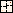
\includegraphics[width=0.3\linewidth, keepaspectratio]{four_rooms.png}
\decoRule
\caption{Another classical MDP: four rooms GridWorld. The agent starts in bottom left room, and the only reward is in the top right one. It can move in all four directions, except there's a $1/3$ chance of actually going in an other direction. The common set of options (see Section \ref{subsec:options}) to consider is moving from one hallway to an other.}
\label{fig:4rooms}
\end{figure}


In decision making problems, an \emph{agent} moves stochastically from state to state in an MDP by taking actions, and depending on its trajectory and decisions receives rewards along the way. This generates a \textbf{history} of transitions $(s_i, a_i, r_i)_{i \in \mathcal{N}}$. Hence the goal is to learn a (near-)optimal decision rule to maximise the rewards, from such history/ies. The agent starts from an initial state based on an \emph{initial distribution} $\mu_0 \in \mathbf{\Delta}(\mathcal{S})$.

A decision rule is defined as a \emph{policy} $\pi : \mathcal{S} \to \Delta(\mathcal{A})$, where $\Delta(\mathcal{A})$ is the set of probability measures over $\mathcal{A}$. $\pi$ is \emph{deterministic} if it maps each state to only one action: $\pi : \mathcal{S} \to \mathcal{A}$. And a policy is \emph{stationary} if it does not depend on the current time step.

Following one stationary policy on $\mathcal{M}$ induces a Markov Reward Process, which is a Markov Chain with rewards upon transitions. In this case, the transition probability kernel follows $\mathbb{P}^\pi(s' \,|\, s) = \mathbb{P}(s' \,|\, s, \pi(s))$.

This link with Markov Chains leads to the following definitions:

\begin{defi}[Classification of MDPs]
  As explained in \citep{fruit_thesis_2019}, Definition 2.2,  a MDP is:
  \begin{enumerate}
  \item \textbf{Ergodic} if the Markov Chain induced by any deterministic stationary policy is ergodic
  \item \textbf{Unichain} if the Markov Chain induced by any deterministic stationary policy is composed of one ergodic sub-Markov Chain in addition to a set of transient states
  \item \textbf{Communicating} if there exists a deterministic stationary policy such that the induced Markov Chain is communicating
  \end{enumerate}
\end{defi}

The ergodic property ensure that, whatever the policy used during learning, all states will be visited infinitely often; unichain means ergodicity except for some states that will not be visited anymore as times goes; and communicating ensure the existence of a path between every pair of states.

\subsection{Settings}
\label{subsec:MDP-settings}

As said before, the goal is to learn to make the best decisions, in other words to find a (near-)optimal policy; however different learning settings exist and are considered in the literature.

A control problem over a MDP is \emph{finite horizon} if only the $H$ first steps are considered, with $H \in \mathbb{N}^*$. Otherwise it is \emph{infinite horizon}. This difference is obviously significative, as the value of a state might change if future rewards can't be obtained because of a finite horizon. The initial state distribution is particularly important in this case, since a high distance from the initial state can make a profitable state not worth it/possible to get to.

A variant of those settings is the \emph{episodic} problem: the agent plays forever, but every $H$ steps it is teleported back to an initial state accordingly to $\mu_0$. It is different from finite horizon since the agent plays this game not just once but infinitely many times, and it is different from infinite horizon as the agent is ``tied'' to those initial states.

Another parameter of such problems is the \emph{discount factor} $\gamma \in [0, 1]$. This is a multiplicative discount applied to rewards based on the time at which they are received, i.e. the reward $r_t$ is actually perceived as $\gamma^t r_t$ by the agent. The motivation behind a discount factor is mathematical, displayed in the next subsection, but intuitively the idea is to penalise long-term reward because of the uncertainty of getting them, while short-term rewards are more reliable. The choice of $\gamma$ is crucial as it is involved in the complexity bounds of many algorithms; as a rule of thumb, we will see that in the discounted setting, $1/(1 - \gamma)$ can be seen as the \emph{effective horizon} of the problem.

\subsection{Measures of performance}
\label{subsec:MDP-measures}

As there are different possible learning settings, there are different possible learning objectives.

The most common one is maximising the \emph{cumulative reward}:

\begin{defi}[Cumulative reward]
  Given a sequence of transitions $(s_t, a_t, r_t)_t$ from an agent in a MDP, we define the cumulative reward $R$ as being:
  \begin{enumerate}
  \item In the finite horizon setting: $\sum_{t=0}^{H}r_t$
  \item In the infinite horizon discounted setting: $\sum_{t=0}^{+\infty} \gamma^t r_t$
  \item In the infinite horizon undiscounted setting: $\liminf_{T \to \+\infty} \frac{1}{T}\sum_{t=1}^{T} r_t$
  \end{enumerate}
  The last definition is more known as the \emph{gain/long-term average reward}, and requires the use of a $\liminf$ to ensure good definition. It represents the asymptotic per-step average reward.\\
  In the infinite horizon undiscounted setting, one can easily see that, since $0 \leq r \leq 1$, $R \leq \frac{1}{1 - \gamma}$; this justifies the use of a discount factor strictly less than one for infinite horizon, otherwise the cumulative reward might diverge.
\end{defi}

When analysing algorithms performances, theoretical results often focus on the \emph{expected cumulative reward}, which is simply the expectation of the cumulative reward.\\[1.5\lineskip]

From now on, \textbf{we shall focus on the finite case infinite horizon discounted setting}.\\[1.5\lineskip]

A more insightful measure is the \emph{regret}: $$\sum_{t=0}^{+\infty} \gamma^t(r_t - r_t^*)$$where $r_t^*$ is the optimal expected reward at time $t$ (the expected reward when taking the optimal action in state $s_t$).

However, while those quantities focus on the ability of the agent to get a lot rewards, one might be more interested in minimising the time needed to learn an $\epsilon$-optimal policy. The $(\epsilon, \delta)$ sample complexity of an agent is the number of time steps $T$ needed before $\| \mathbf{V}_t^\pi - \mathbf{V}^* \|_\infty \leq \epsilon$ for all $t \geq T$ with probability $1 - \delta$, where $\mathbf{V}_t^\pi$ is the value of the policy of the agent at step $t$ and $\mathbf{V}^*$ is the optimal value (values are defined in the next section). Intuitively, this is the PAC convergence speed to a policy.

Finally, another version of sample complexity is the (asymptotic) upper-bound on the number of steps where the current policy isn't $\epsilon$-optimal. In this case, the emphasis is put on minimising the number of mistakes rather than on the learning speed.

Now we shall introduce some crucial notion with respect to those measures of learning performance.

\subsection{Values \& Optimality}
\label{subsec:MDP-values}

In order to get to optimality, many MPD algorithms assign values to states or state-action pairs. These quantities guide decision making towards the most profitable choice, and allow to progressively improve the value of a policy.

\begin{defi}[Value \& Q-value]
  For any policy $\pi$, we define for all state-action pair $(s, a) \in \mathcal{S}\times \mathcal{A}$:
  \begin{align*}
  V^\pi(s) &= \mathbb{E}_\pi \left[\sum_{t=0}^{+\infty} \gamma^t r(s_t, a_t) \,|\, s_0=s \right]\\
  Q(s, a)^\pi &= \mathbb{E}_\pi \left[\sum_{t=0}^{+\infty} \gamma^t r(s_t, a_t) \,|\, s_0=s, a_0=a \right]
  \end{align*}
  From these definitions, one can see that $V^\pi(s) = Q(s, \pi(s))$.
  The \textbf{value} and the \textbf{Q-value} functions of $\pi$, respectively. The expectation $\mathbb{E}_\pi[\dots]$ means that the actions $a_t$ are taking accordingly to $\pi(s_t)$.\\
  In the finite case, we denote $\mathbf{V}^\pi$ and $\mathbf{Q}^\pi$ the vectors of values and Q-values of $\pi$.
\end{defi}

As one can see, those quantities represent what an agent can expect to get as rewards in the future, from its current state/state-action. The value can guide the decision making, as with the \emph{greedy policy} $\pi_g(s) = \arg\max_{a \in \mathcal{A}} Q(s, a)$. From here, it is easy to define what an \emph{optimal} policy is:

\begin{defi}[Optimality]
  A policy $\pi^*$ is optimal if $$\forall \, s \in \mathcal{S},\quad \pi^* \in \arg\max_{\pi \in \Pi} V^\pi(s)$$ where $\Pi$ is the set of all policies.\\
  We then denote $V^{\pi^*} = V^*$, the optimal state value function.\\
  Similarly, $Q^{\pi^*} = Q^*$ and $V^*(s) = \max_{a \in \mathcal{A}} Q^*(s, a)$ for all $s \in \mathcal{S}$.\\
  Moreover, there exists one optimal policy $\pi^*_d$ that is deterministic, and $\pi^*_d(s) = \arg\max_{a \in \mathcal{A}} Q^*(s,a)$ for all $s \in \mathcal{S}$.
\end{defi}

One can already see how relevant the value of a policy is when seeking optimality, but what makes those functions so interesting is the following property:

\begin{defi}[Bellman operator]
  The Bellman operator \citep{bellman1957markovian} associated to a policy $\pi$ is $$\mathcal{T}^\pi : \begin{cases} &\mathbb{R}^S \to \mathbb{R}^S\\ V &\mapsto \mathcal{T}^\pi(V) \end{cases}$$ where $$\forall \, s \in \mathcal{S},\quad \mathcal{T}^\pi(V)(s) = r(s, \pi(s)) + \gamma \sum_{s'\in \mathcal{S}} p(s' \,|\, s, \pi(s)) V(s')$$
  $\mathcal{T}^\pi$ being a $\gamma$-contraction, $V^\pi$ is the only fixed point \citep{blackwell1962discrete}: $$\forall \, s \in \mathcal{S},\quad V^\pi(s) = r(s, \pi(s)) + \gamma \sum_{s'\in \mathcal{S}} p(s' \,|\, s, \pi(s)) V^\pi(s')$$\\
  Thanks to this result, the greedy policy can be obtained from $V$: $$\pi_g(s) = \arg\max_{a \in \mathcal{A}} \left[ r(s,a) + \gamma \sum_{s' \in \mathcal{S}}p(s' \,|\, s, a) V^*(s') \right]$$
  A similar result holds for the Q-value: $$\forall \, (s, a) \in \mathcal{S}\times \mathcal{A},\quad Q^\pi(s, a) = \mathcal{T}^\pi(Q)(s,a) = r(s, a) + \gamma \sum_{s' \in \mathcal{S}} p(s \,|\, s,a) V^\pi (s')$$
  When considering any optimal policy, one get the \textbf{optimal Bellman operator}: $$\mathcal{T}^*(V)(s) = \max_{a \in \mathcal{A}} \left[ r(s, a) + \gamma \sum_{s' \in \mathcal{S}} p(s' \,|\, s,a)V(s') \right]$$
  Since $\mathcal{T}^*$ is a $\gamma$-contraction as well, iteratively applying $\mathcal{T}^*$ over an initial value function $V_0$ converges towards $V^*$.
\end{defi}

As the reader can realise from the above properties of the Bellman operator, we just acquired a great theoretical tool on our way towards optimality. The significance of the Bellman operator is showcased in the following section.


\section{Reinforcement Learning basics}
\label{section:RL}

In this section, we shall present the basic approaches to solve a MDP problem. While those algorithms have been knwon for some time already, they still represent the foundation of many of the latest ones, and are still actively studied.

\subsection{Planning}
\label{subsec:RL-planning}

Actually preceding Reinforcement Learning is the field of \emph{planning}: planning is the problem of seeking optimality when the MDP is fully known, specifically $p$ and $r$. The results introduced in the previous section allow us to directly present \emph{Value Iteration} (algorithm \ref{alg:VI}).

\begin{algorithm}[htbp]
\small
\caption{Value Iteration}
\label{alg:VI}
\begin{algorithmic}
\State \textbf{Initialization:} $\mathbf{V_0} \in \mathbb{R}^S$ initial value, $\epsilon > 0$ error margin.
\State $\mathbf{V} \leftarrow \mathbf{V_0}$
\While{$\| \mathbf{V} - \mathcal{T}^*(\mathbf{V}) \|_\infty \geq \epsilon$}
\State $\mathbf{V} \leftarrow \mathcal{T}^*(\mathbf{V})$
\EndWhile\State
\Return $\pi_g$ the greedy algorithm with respect to $\mathbf{V}$.
\end{algorithmic}
\normalsize
\end{algorithm}

In this approach, the optimisation is done in the world of the value functions, and an optimal policy is obtained with the greedy operator. The next algorithm though, \emph{Policy Iteration} (algorithm \ref{alg:PI}), operates directly on the world of policies via evaluation and then improvement from the evaluation.

\begin{algorithm}[htbp]
\small
\caption{Policy Iteration}
\label{alg:PI}
\begin{algorithmic}
\State \textbf{Initialization:} $\pi_0 \in \Pi$ intial policy.
\State $\pi_1 \leftarrow \pi_0$
\State $\pi_2 \leftarrow \emptyset$
\While{$\pi_1 \neq \pi_2$}
\State $\pi_2 \leftarrow \pi_1$
\State Compute/estimate $V^{\pi_1}$ \Comment{Policy evalutation}
\State $\pi_1 \leftarrow \mathsf{greedy}(V^{\pi_1})$ \Comment{Policy improvement}
\EndWhile\State
\Return $\pi_1$
\end{algorithmic}
\normalsize
\end{algorithm}


It is interesting to notice how the Policy Iteration requires a policy evaluation algorithm (such as Value Iteration); this highlight the power of value functions.

\subsection{Various Reinforcement Learning paradigms}
\label{subsec:RL-paradigms}

However in real-world application, one is more often interested in Reinforcement Learning problems, where \emph{$r$ and $p$ are unknown} ($\mathcal{S}$ and $\mathcal{A}$ can usually be assumed to be known). Because of this lack of knowledge, the previous algorithms can't be used right away. To handle this difficulty, many strategies have been developped.

First of all, we can distinguish \emph{model-free} and \emph{model-based} algorithms: in the latter, estimates of $p$ and $r$ are first computed, and then used in a planning algorithm; while a model-free approach directly estimates values or policies.

To build those estimates, multiple techniques are possible, such as Monte-Carlo or Temporal Difference. However, Monte-Carlo methods require a significant number of simulations that grows with $S$ and $A$ to work, while on the contrary Temporal Difference updates use very little data, thus possibly missing some crucial information on the MDP. In that respect, an interesting notion is the \emph{Optimism in the face of Uncertainty}: adding a bias in estimates that favors least explored states. This illustrates the \emph{Exploration-Exploitation} trade-off problem in online learning: exploration is costly but necessary to take good decisions. Another example is the use of the \emph{$\epsilon$-greedy} policy, where with probability $\epsilon$ a random action is taken, otherwise the greedy action is followed.

Furthermore, a RL algorithm is said to be either \emph{on-policy} or \emph{off-policy}: in the first case, the policy used to simulate and collect samples is the policy improved and returned, while in the second case a \emph{behavior policy} is followed during execution while the data is used to improve the target policy.

These ideas are showcased in the enxt subsection.

\subsection{Q-Learning}
\label{subsec:Rl-QL}

Q-Learning (QL) is one of the oldest and most important algorithm in RL \citep{watkins1989learning}. Indeed, numerous variants have been proposed since, and proofs for theoretical guarantees are still being published nowadays.

QL is a model-free off-policy that uses Temporal Difference updates to maintain an estimate of $Q^*$, which then can be used to get $\pi^*$. It is very simple, as shown in algorithm \ref{alg:QL}.

\begin{algorithm}[htbp]
\small
\caption{Asynchronous Q-Learning}
\label{alg:QL}
\begin{algorithmic}
\State \textbf{Initialization:} $\pi_b \in \Pi$ behaviour policy, $(\alpha_i)_{i \in \mathbb{N}}$ learning rates, $Q_0 \in \mathbb{R}^{S \times A}$ initial Q-value matrix, $s_0$ initial state, $N_0(s,a) = 0 \ \forall (s,a)$ the number of visits of $(s,a)$ so far.
\For{$t=1,2,\ldots$}
\State Sample action $a_t\sim \pi_b(s_t)$ and observe $s_{t+1}\sim P(\cdot\vert s_t,a_t)$.
\State $N_{t+1}(s_t,a_t)=N_t(s_t,a_t)+1$
\State $\alpha = \alpha_{N_t(s_t,a_t)+1}$
\State $Q_{t+1}(s_t,a_t)= (1-\alpha)Q_t(s_t,a_t)+\alpha\Big(r(s_t,a_t)+\gamma \max_{a\in\mathcal{A}}Q_t(s_{t+1},a)\Big)$.
\EndFor
\end{algorithmic}
\normalsize
\end{algorithm}

In synchronous QL, the behaviour policy is replaced by $\mathbf{greedy}(Q_t)$, or $\epsilon-\mathbf{greedy}(Q_t)$ to keep on exploring. Also, many tweaks can be made such as using optimistic initial values or maintaining two estimates of $Q$ \citep{even-dar_convergence_2001, hasselt2010double}. A common choice for the learning rate is $\alpha_i = \frac{1}{i}$.

The core idea of Temporal Difference is that $r(s_t,a_t)+\gamma \max_{a\in\mathcal{A}}Q_t(s_{t+1},a) = \mathcal{T}^*(Q)(s,a)$ is actually an estimate of $Q^*$.

\begin{thm}[Convergence of Q-Learning \citep{jaakkola1994reinforcement}]\label{thm:QL-conv}
  If all state-action pairs are visited infinitely often and $$\sum_{i=1}^{+\infty}\alpha_i = +\infty \quad\text{and}\quad \sum_{i=1}^{+\infty}\alpha_i^2 < +\infty$$ then $Q_t$ will converge to $Q^*$ with probability 1 as $t$ tends towards infinity.
\end{thm}

This result justify the QL algorithm. However, it is very well known that, even if the QL update is very cheap to execute, the convergence can be very slow, hence QL is not \emph{sample efficient}.

Please note that for all state-action pairs to be visited infinitely often is equivalent to say that the Markov Chain induced by $\pi_b$ is ergodic.
